\documentclass{standalone}
\usepackage{tikz}
\usetikzlibrary{patterns, positioning}

\begin{document}
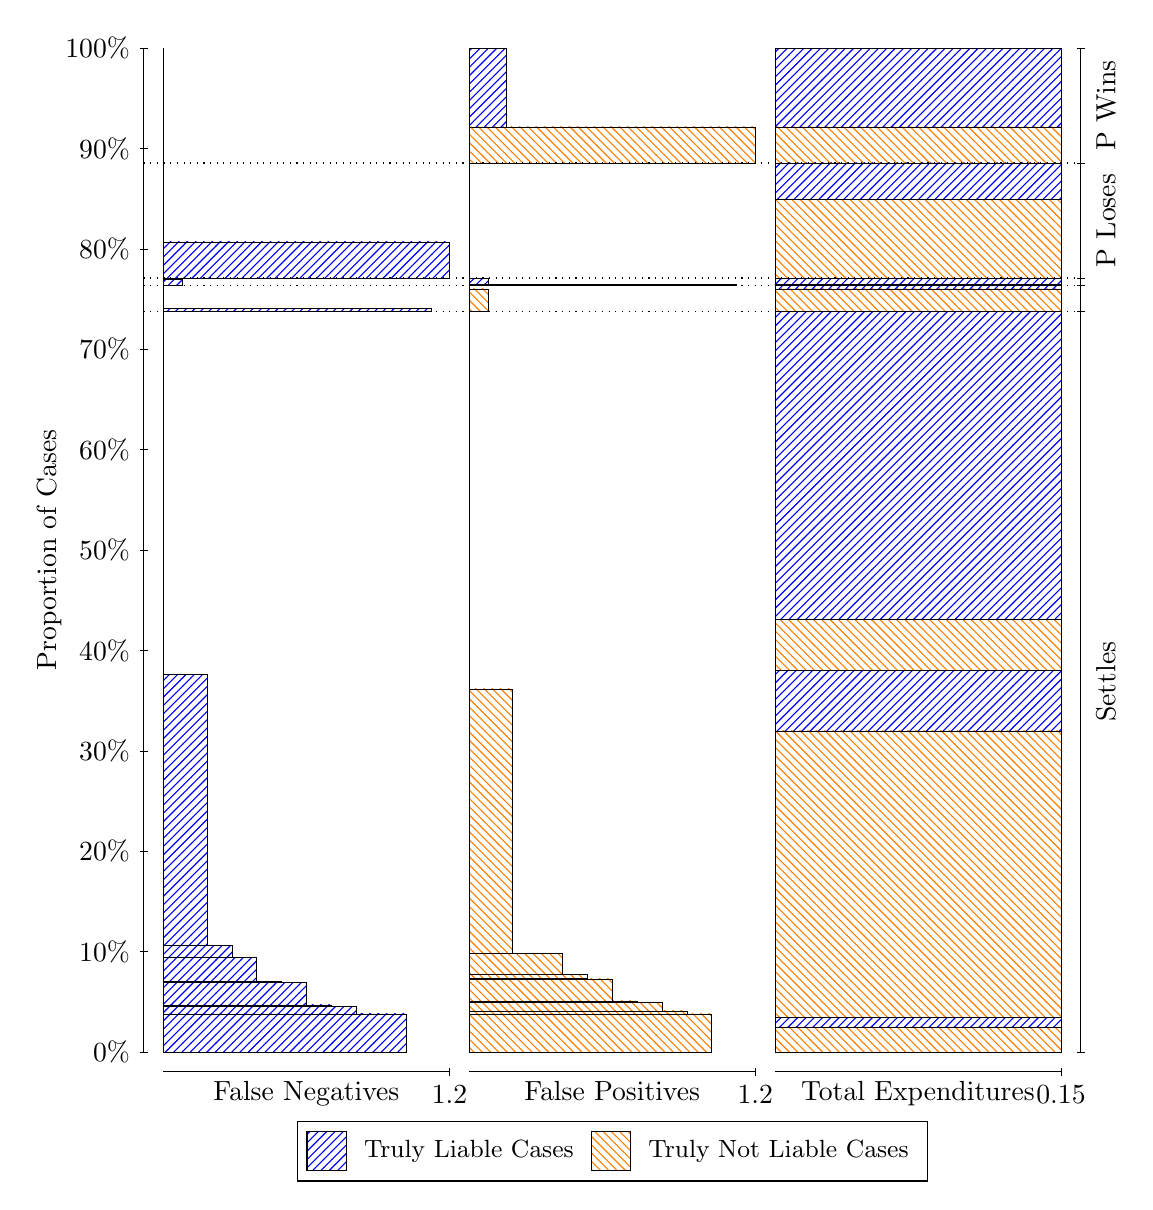
\begin{tikzpicture}
\draw[black, very thin] (1.5,1.75) -- (1.5,14.5);
\node[rotate=90, anchor=center] at (0.3, 8.125) {Proportion of Cases};
\draw[black, very thin] (1.45,1.75) -- (1.55,1.75);
\node[anchor=east] at (1.45, 1.75) {0\%};
\draw[black, very thin] (1.45,3.025) -- (1.55,3.025);
\node[anchor=east] at (1.45, 3.025) {10\%};
\draw[black, very thin] (1.45,4.3) -- (1.55,4.3);
\node[anchor=east] at (1.45, 4.3) {20\%};
\draw[black, very thin] (1.45,5.575) -- (1.55,5.575);
\node[anchor=east] at (1.45, 5.575) {30\%};
\draw[black, very thin] (1.45,6.85) -- (1.55,6.85);
\node[anchor=east] at (1.45, 6.85) {40\%};
\draw[black, very thin] (1.45,8.125) -- (1.55,8.125);
\node[anchor=east] at (1.45, 8.125) {50\%};
\draw[black, very thin] (1.45,9.4) -- (1.55,9.4);
\node[anchor=east] at (1.45, 9.4) {60\%};
\draw[black, very thin] (1.45,10.675) -- (1.55,10.675);
\node[anchor=east] at (1.45, 10.675) {70\%};
\draw[black, very thin] (1.45,11.95) -- (1.55,11.95);
\node[anchor=east] at (1.45, 11.95) {80\%};
\draw[black, very thin] (1.45,13.225) -- (1.55,13.225);
\node[anchor=east] at (1.45, 13.225) {90\%};
\draw[black, very thin] (1.45,14.5) -- (1.55,14.5);
\node[anchor=east] at (1.45, 14.5) {100\%};

\draw[black, very thin] (13.4,1.75) -- (13.4,14.5);
\draw[black, very thin] (13.35,1.75) -- (13.45,1.75);
\node[anchor=west] at (13.35, 1.75) {};
\draw[black, very thin] (13.35,11.154) -- (13.45,11.154);
\node[anchor=west] at (13.35, 11.154) {};
\draw[black, very thin] (13.35,11.481) -- (13.45,11.481);
\node[anchor=west] at (13.35, 11.481) {};
\draw[black, very thin] (13.35,11.579) -- (13.45,11.579);
\node[anchor=west] at (13.35, 11.579) {};
\draw[black, very thin] (13.35,13.04) -- (13.45,13.04);
\node[anchor=west] at (13.35, 13.04) {};
\draw[black, very thin] (13.35,14.5) -- (13.45,14.5);
\node[anchor=west] at (13.35, 14.5) {};

\draw[black, very thin, pattern color=blue, pattern=north east lines] (1.75,1.75) rectangle (4.8304,2.2335);
\draw[black, very thin, pattern color=blue, pattern=north east lines] (1.75,2.2335) rectangle (4.5145,2.235);
\draw[black, very thin, pattern color=blue, pattern=north east lines] (1.75,2.235) rectangle (4.1986,2.3301);
\draw[black, very thin, pattern color=blue, pattern=north east lines] (1.75,2.3301) rectangle (3.8826,2.3493);
\draw[black, very thin, pattern color=blue, pattern=north east lines] (1.75,2.3493) rectangle (3.5667,2.6302);
\draw[black, very thin, pattern color=blue, pattern=north east lines] (1.75,2.6302) rectangle (3.2507,2.6467);
\draw[black, very thin, pattern color=blue, pattern=north east lines] (1.75,2.6467) rectangle (2.9348,2.9498);
\draw[black, very thin, pattern color=blue, pattern=north east lines] (1.75,2.9498) rectangle (2.6188,3.1015);
\draw[black, very thin, pattern color=blue, pattern=north east lines] (1.75,3.1015) rectangle (2.3029,6.5435);
\draw[black, very thin, pattern color=orange, pattern=north west lines] (1.75,6.5435) rectangle (1.75,11.154);
\draw[black, very thin, pattern color=blue, pattern=north east lines] (1.75,11.154) rectangle (5.1464,11.194);
\draw[black, very thin, pattern color=orange, pattern=north west lines] (1.75,11.194) rectangle (1.75,11.481);
\draw[black, very thin, pattern color=blue, pattern=north east lines] (1.75,11.481) rectangle (1.987,11.562);
\draw[black, very thin, pattern color=orange, pattern=north west lines] (1.75,11.562) rectangle (1.75,11.579);
\draw[black, very thin, pattern color=blue, pattern=north east lines] (1.75,11.579) rectangle (5.3833,12.037);
\draw[black, very thin, pattern color=orange, pattern=north west lines] (1.75,12.037) rectangle (1.75,13.04);
\draw[black, very thin, pattern color=orange, pattern=north west lines] (1.75,13.04) rectangle (1.75,13.499);
\draw[black, very thin, pattern color=blue, pattern=north east lines] (1.75,13.499) rectangle (1.75,14.5);
\draw[black, very thin, pattern color=orange, pattern=north west lines] (5.6333,1.75) rectangle (8.7138,2.2347);
\draw[black, very thin, pattern color=orange, pattern=north west lines] (5.6333,2.2347) rectangle (8.3978,2.2718);
\draw[black, very thin, pattern color=orange, pattern=north west lines] (5.6333,2.2718) rectangle (8.0819,2.382);
\draw[black, very thin, pattern color=orange, pattern=north west lines] (5.6333,2.382) rectangle (7.7659,2.3979);
\draw[black, very thin, pattern color=orange, pattern=north west lines] (5.6333,2.3979) rectangle (7.45,2.6794);
\draw[black, very thin, pattern color=orange, pattern=north west lines] (5.6333,2.6794) rectangle (7.1341,2.6846);
\draw[black, very thin, pattern color=orange, pattern=north west lines] (5.6333,2.6846) rectangle (7.1341,2.7306);
\draw[black, very thin, pattern color=orange, pattern=north west lines] (5.6333,2.7306) rectangle (6.8181,2.9976);
\draw[black, very thin, pattern color=orange, pattern=north west lines] (5.6333,2.9976) rectangle (6.5022,2.9995);
\draw[black, very thin, pattern color=orange, pattern=north west lines] (5.6333,2.9995) rectangle (6.1862,6.36);
\draw[black, very thin, pattern color=blue, pattern=north east lines] (5.6333,6.36) rectangle (5.6333,11.154);
\draw[black, very thin, pattern color=orange, pattern=north west lines] (5.6333,11.154) rectangle (5.8703,11.441);
\draw[black, very thin, pattern color=blue, pattern=north east lines] (5.6333,11.441) rectangle (5.6333,11.481);
\draw[black, very thin, pattern color=orange, pattern=north west lines] (5.6333,11.481) rectangle (9.0297,11.498);
\draw[black, very thin, pattern color=blue, pattern=north east lines] (5.6333,11.498) rectangle (5.8703,11.579);
\draw[black, very thin, pattern color=orange, pattern=north west lines] (5.6333,11.579) rectangle (5.6333,12.581);
\draw[black, very thin, pattern color=blue, pattern=north east lines] (5.6333,12.581) rectangle (5.6333,13.04);
\draw[black, very thin, pattern color=orange, pattern=north west lines] (5.6333,13.04) rectangle (9.2667,13.499);
\draw[black, very thin, pattern color=blue, pattern=north east lines] (5.6333,13.499) rectangle (6.1072,14.5);
\draw[black, very thin, pattern color=orange, pattern=north west lines] (9.5167,1.75) rectangle (13.15,2.07);
\draw[black, very thin, pattern color=blue, pattern=north east lines] (9.5167,2.07) rectangle (13.15,2.1859);
\draw[black, very thin, pattern color=orange, pattern=north west lines] (9.5167,2.1859) rectangle (13.15,5.828);
\draw[black, very thin, pattern color=blue, pattern=north east lines] (9.5167,5.828) rectangle (13.15,6.5923);
\draw[black, very thin, pattern color=orange, pattern=north west lines] (9.5167,6.5923) rectangle (13.15,7.2402);
\draw[black, very thin, pattern color=blue, pattern=north east lines] (9.5167,7.2402) rectangle (13.15,11.154);
\draw[black, very thin, pattern color=orange, pattern=north west lines] (9.5167,11.154) rectangle (13.15,11.441);
\draw[black, very thin, pattern color=blue, pattern=north east lines] (9.5167,11.441) rectangle (13.15,11.481);
\draw[black, very thin, pattern color=orange, pattern=north west lines] (9.5167,11.481) rectangle (13.15,11.498);
\draw[black, very thin, pattern color=blue, pattern=north east lines] (9.5167,11.498) rectangle (13.15,11.579);
\draw[black, very thin, pattern color=orange, pattern=north west lines] (9.5167,11.579) rectangle (13.15,12.581);
\draw[black, very thin, pattern color=blue, pattern=north east lines] (9.5167,12.581) rectangle (13.15,13.04);
\draw[black, very thin, pattern color=orange, pattern=north west lines] (9.5167,13.04) rectangle (13.15,13.499);
\draw[black, very thin, pattern color=blue, pattern=north east lines] (9.5167,13.499) rectangle (13.15,14.5);
\draw[black, dotted] (1.5,11.154) -- (13.4,11.154);
\draw[black, dotted] (1.5,11.481) -- (13.4,11.481);
\draw[black, dotted] (1.5,11.579) -- (13.4,11.579);
\draw[black, dotted] (1.5,13.04) -- (13.4,13.04);
\draw[black, very thin] (1.75,1.5) -- (5.3833,1.5);
\node[anchor=north] at (3.5667, 1.5) {False Negatives};
\draw[black, very thin] (5.3833,1.45) -- (5.3833,1.55);
\node[anchor=north] at (5.3833, 1.45) {1.2};

\draw[black, very thin] (5.6333,1.5) -- (9.2667,1.5);
\node[anchor=north] at (7.45, 1.5) {False Positives};
\draw[black, very thin] (9.2667,1.45) -- (9.2667,1.55);
\node[anchor=north] at (9.2667, 1.45) {1.2};

\draw[black, very thin] (9.5167,1.5) -- (13.15,1.5);
\node[anchor=north] at (11.333, 1.5) {Total Expenditures};
\draw[black, very thin] (13.15,1.45) -- (13.15,1.55);
\node[anchor=north] at (13.15, 1.45) {0.15};

\node[black, centered, rotate=90] at (13.72, 6.4518) {Settles};


\node[black, centered, rotate=90] at (13.72, 12.309) {P Loses};
\node[black, centered, rotate=90] at (13.72, 13.77) {P Wins};

\draw (7.449999999999999,1.5) node[draw=none] (baseCoordinate) {};
\begin{scope}[align=center]
        \matrix[scale=0.5, draw=black, below=0.5cm of baseCoordinate, nodes={draw}, column sep=0.1cm]{
            \node[rectangle, draw, minimum width=0.5cm, minimum height=0.5cm, pattern=north east lines, pattern color=blue] {}; &
            \node[draw=none, font=\small] (B) {Truly Liable Cases}; &
            \node[rectangle, draw, minimum width=0.5cm, minimum height=0.5cm, pattern=north west lines, pattern color=orange] {}; &
            \node[draw=none, font=\small] (B) {Truly Not Liable Cases}; \\
            };
\end{scope}

\end{tikzpicture}
\end{document}